% !TeX spellcheck = en_US
\chapter{Introduction}
\label{ch:intro}

\section{Terminology}
\label{sec:terminology}

A \textbf{system} is the portion of the world affected by the decision, it should allow different configurations, it should not be given once and for all, otherwise no decision would be possible. 

A \textbf{solution} or \textbf{alternative} is the combination of all controllable aspects of the system, and \textbf{outcome} or \textbf{scenario} the combination of all its uncontrollable aspects. 

A system combines controllable and uncontrollable aspects into a \textbf{configuration}. Each configuration is associated to an \textbf{impact}, that describes all aspects relevant for the decision.

\textbf{Decision-maker} or \textbf{stakeholder} refers to everybody who contributes to the choice of the alternative. The former indicates who takes part to the choice, while the latter also includes who does not participate but has interests at stake and could react to a disagreeable choice, exerting an indirect influence on the choice. 

With \textbf{preference}, we denote the relative satisfaction between impacts. 

A decision problem requires to \textit{choose an alternative}: 
\begin{itemize}
	\item so as to \textit{move the system into a configuration} 
	
	\item such that \textit{the decision-makers prefers its associated impact} to those of other configurations
	
	\item keeping into account that \textit{the actual configuration depends on the alternative, but also on the scenario}
\end{itemize}

A \textbf{decision problem} implies two fundamental conditions: 
\begin{itemize}
	\item \textbf{Freedom}, i.e., availability of different choices (otherwise there is no decision)
	
	\item \textbf{Rationality}, i.e., the existence of preference criteria (otherwise the choice cannot be motivated)
\end{itemize}

This is a concept different from the definition of "decision problem" typically given in computer science (problem which admits only two possible solutions, \textit{yes} or \textit{no}). The decision problems considered here can be considered special cases of optimization/search problems, whose solution is an object with the maximum value (or minimum cost). 

%TODO Check
The focus is on practical decisions where a large amount of data must be taken into account, many choices are possible and the cost of a wrong choice is high.

We want to discuss \textit{what makes a decision complicated}, present the mathematical models to describe complicated situations and present the methods to deal with such situations, while recognizing limits and errors of this approach.

\section{Modeling approach to decision}
\label{sec:modelingapproach}

The modeling approach to decision requires a series of intermediate passages: 
\begin{itemize}
	\item Building a model of the problem
	
	\item Solving the model with algorithms, i.e., formal methods
	
	\item Interpreting the solution, with suitable methods
\end{itemize}

The strategy is to first \textbf{make a model}, then \textbf{compute}, and \textbf{finally decide}. From a problem to a model, solved by an algorithm, then actions are taken based on the solution.

The \textbf{decision process} occurs in an \textbf{iterative correction approach}:
\begin{enumerate}
	\item \textit{Problem formulation:} delineate the system, identifying impacts and preferences (Objectives) on one hand, decision-makers and scenarios (Context) on the other
	
	\item \textit{Alternative identification:} define the set of feasible alternatives
	
	\item \textit{Alternative evaluation and choice:} evaluate the impact associated to each configuration (alternative and scenario) and choose an alternative based on the preferences of the decision-makers
	
	\item \textit{Decision implementation:} apply or simulate the alternative selected
	
	\item \textit{Monitoring and check:} observe the consequences of the decision; if unsatisfactory, make correction and repeat the process, introducing new scenarios, objectives, alternatives and evaluation methods
\end{enumerate}

\begin{center}
	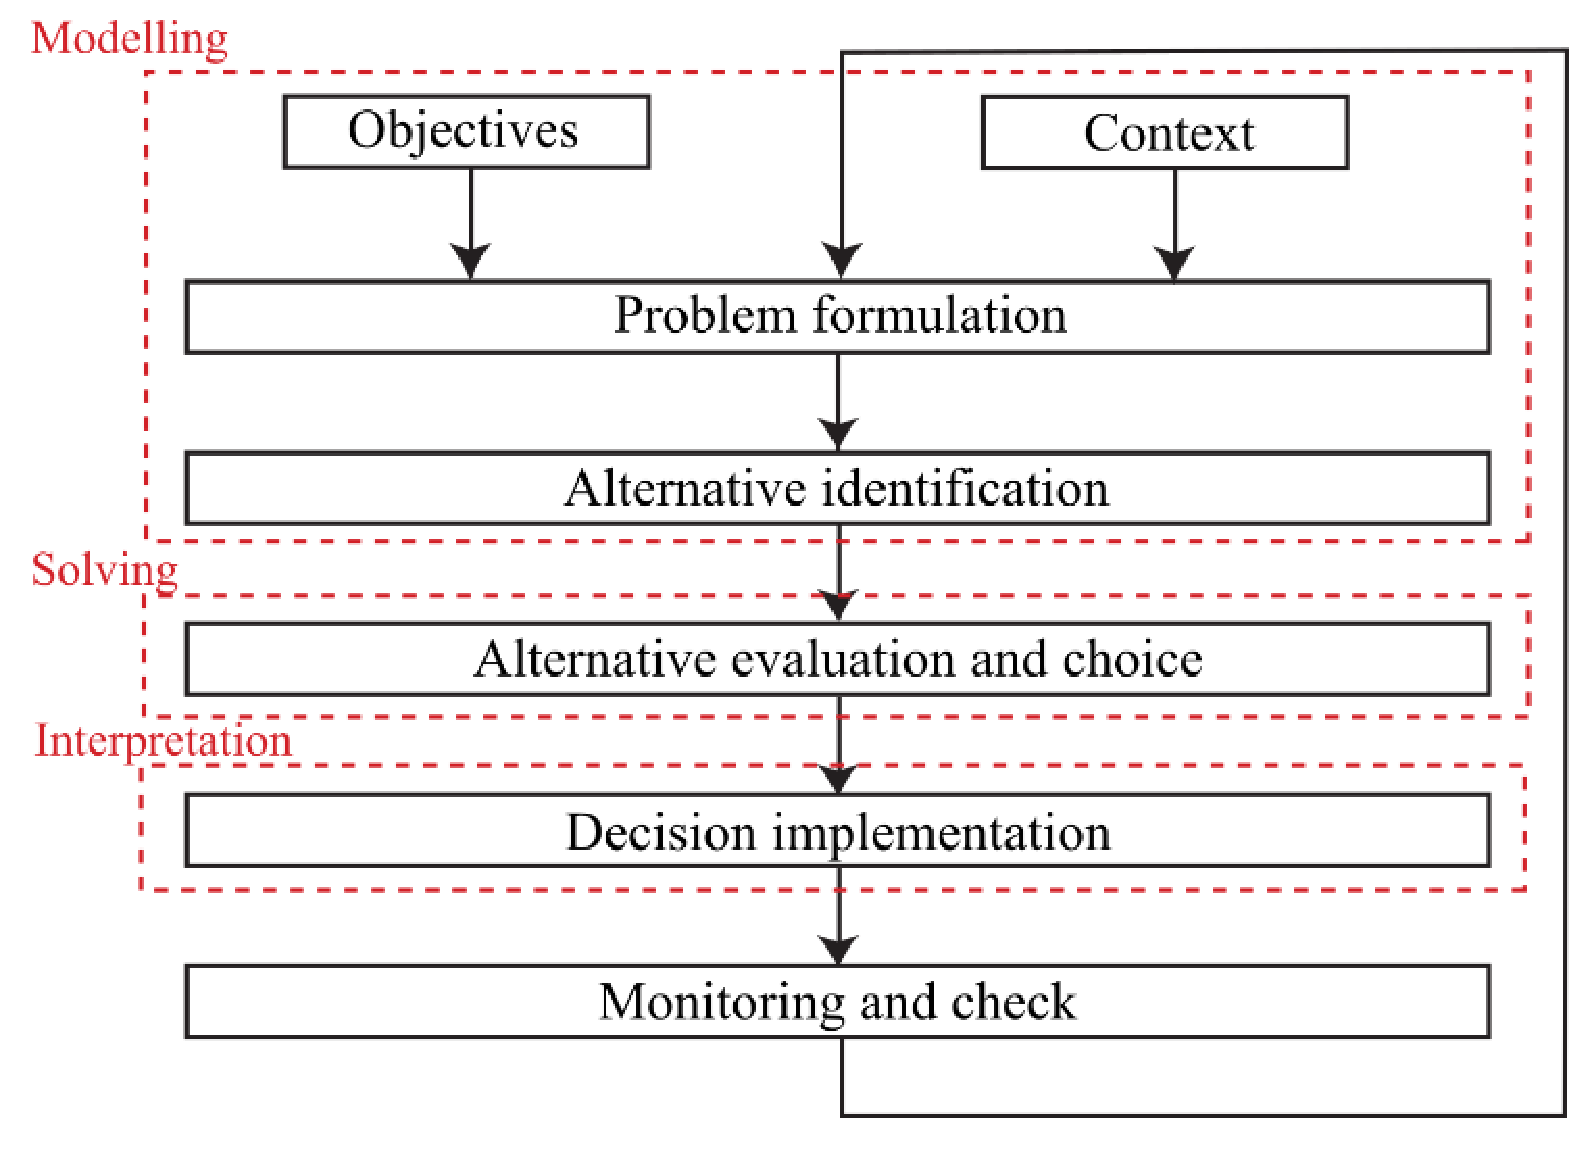
\includegraphics[width=0.75\columnwidth]{img/dp/intro/decisionIter}
\end{center}

\section{Why a formal approach?}
\label{sec:whyformal}

A formal approach allows to: 
\begin{itemize}
	\item Predict in a more certain and precise way the impact of a decision, using descriptive models instead of intuition and experience
	
	\item Accelerate the decision process, using algorithms and information technology
	
	\item Consider a much larger number of possible alternatives
	
	\item Clarifying and certifying the decision process
	\begin{itemize}
		\item making explicit the assumptions made on alternatives, scenarios, preferences and decision-makers
		
		\item guaranteeing repeatability of the process 
		
		\item allowing specific changes to the process, without starting from scratch
	\end{itemize}
\end{itemize}

The formal approach is based on
\begin{itemize}
	\item \textbf{Models}, to take decisions and predict their outcomes
	
	\item \textbf{Methods}, to build models, solve them, and interpret their results
\end{itemize}

\section{Prescriptive and descriptive models}
\label{sec:prescriptivedescriptive}

A decision model includes a number of sub-models, which can be classified based on the data they require and the result they produce. Decision models usually combine:
\begin{enumerate}
	\item \textbf{Prescriptive models} that
	\begin{itemize}
		\item receive impacts and preferences in input
		
		\item return a suggested alternative in output
	\end{itemize}
	\textit{if this is the case, you should do that}
	
	\item \textbf{Descriptive/predictive} models
	\begin{itemize}
		\item receive the system, an alternative and a scenario in input
		
		\item return an impact in output
	\end{itemize}
	\textit{If you do this and if this happens, you will obtain that}
\end{enumerate}

The two families of models can have subtle and complex interactions. For example, any prescriptive model uses a set of descriptive models to obtain the impacts of possible alternatives and scenarios; on the other hand, some descriptive models can include prescriptive ones.

Example: a model prescribes  a decision (\textit{close or open streets}) based on models that describe a system (\textit{amount of traffic}), including decisions prescribed by models (\textit{satellite navigators})

\section{What makes a decision problem complicated?}
\label{whycomplicated}

A decision problem can be \textit{complicated} due to:
\begin{itemize}
	\item An \textbf{insufficient model} of the system
	
	\item \textbf{Complicating features} of the model, such as
	\begin{itemize}
		\item complex preference structure, insufficient to define an optimum
		
		\item uncertain environment, impact depends also on unknown scenario
		
		\item multiple decision-makers, with potentially conflicting preferences
	\end{itemize}
	
	\item A \textbf{computationally complex model}, everything is clearly defined, but no efficient algorithm is known to solve the problem
\end{itemize}

The three main complexity sources for decision problems are: 
\begin{enumerate}
	\item \textbf{Preference structure}: simple or complex
	
	\item \textbf{Uncertainty}: a single scenario or many 
	
	\item \textbf{Decision-makers}: single or many
\end{enumerate}
giving rise to $2^3 = 8$ families of decision problems.

We'll consider four basic families of prescriptive models: 
\begin{enumerate}
	\item Simple preference, a single scenario and a single decision maker:
	\begin{itemize}
		\item mathematical programming
		
		\item multi-attribute utility theory
	\end{itemize}
	
	\item Complex preference, a single scenario and a single decision maker:
	\begin{itemize}
		\item paretian preferences
		
		\item weak rationality models (\textit{AHP} and \textit{ELECTRE} methods)
	\end{itemize}
	
	\item Simple preference, multiple scenarios and a single decision-maker:
	\begin{itemize}
		\item decisions in condition of ignorance (robust programming)
		
		\item decisions in conditions of risk (stochastic programming)
	\end{itemize}
	
	\item Simple preference, a single scenario and multiple decision-makers: 
	\begin{itemize}
		\item independent decision-makers (game theory)
		
		\item cooperating decision-makers (group decisions)
	\end{itemize}
\end{enumerate}

\subsection{Examples of complicated decision problems}
\label{subsec:examplesofcomplicatedproblems}

Before some large-size examples (Chapter \ref{ch:cases}), we present some realistic situations that might suggest what elements make a decision complicated in practice.

\paragraph{\textit{The search for parking:}} In a rather congested town, we are looking for a parking to leave out car and reach the place of an important meeting; we would prefer to park quickly  and not walk for long to reach the destination.
\begin{itemize}
	\item \textit{System} is the local street network, with the set of all potential parking places
	
	\item \textit{Alternative} is every possible trajectory of the car (path and time)
	
	\item \textit{Scenario} is every possible distribution of the free parking spaces over space and time
	
	\item \textit{Impact} are the driving time and walking time after parking
	
	\item \textit{Decision-maker} is the driver
\end{itemize}

The impact reduces to the aspects which actually matter for the decision, but it depends on a complex combination (configuration) of every possible trajectory of the car and distribution of parking spaces (alternative and scenario).

\paragraph{\textit{Thermostat regulation:}} We want to tune the classroom's thermostat so that the temperature is pleasant for the teacher and students.
\begin{itemize}
	\item \textit{System} is the classroom
	
	\item \textit{Alternative} is the position of the thermostat
	
	\item \textit{Scenario} is the external temperature and the exposition of the classroom to the sun 
	
	\item \textit{Impact} is the internal temperature of the classroom (but probably, also the humidity)
	
	\item \textit{Decision-makers} are all the people in the classroom (or just the teacher?)
\end{itemize}

This problem is easier than the others, but the definition of impact and decision-makers is not trivial.

\paragraph{\textit{Buying a car:}} We want to buy a car with good performance, comfort, design and low cost throughout its life cycle.
\begin{itemize}
	\item \textit{System} is the local market of cars, petrol, repairs, etc.
	
	\item \textit{Alternative} is the car bought 
	
	\item \textit{Scenario} are the stock and prices of the car dealers, the occurrence of accidents, prices of petrol and repairs, etc. 
	
	\item \textit{Impact} are the characteristics of the car throughout its life cycle
	
	\item \textit{Decision-maker} is the buyer (possibly some other family members/friends?)
\end{itemize}

A possible alternative, easy to forget, is to not buy a car, with an impact very bad for some aspects, but very good for others.

\paragraph{\textit{Risiko round:}} We want to play a round of Risiko, considering in turn all of the players.
\begin{itemize}
	\item \textit{System} is the map, with the distribution of territories, armies, cards
	
	\item \textit{Alternative} are the territories from which and to which each attack is launched and the corresponding number of attacking and defending armies
	
	\item \textit{Scenario} is the dices' outcome at each attack
	
	\item \textit{Impact} is the number of armies destroyed for each player
	
	\item \textit{Decision-makers} are the players
\end{itemize}

Here the presence of multiple decision-makers is intrinsic and unavoidable, moreover they all make their own choices autonomously.
